\documentclass[12pt]{article}

\usepackage[bottom = 15mm]{geometry}
\usepackage[utf8]{inputenc}
\usepackage[T2A]{fontenc}
\usepackage[russian]{babel}
\usepackage{graphicx}
\usepackage{caption}
\usepackage{amssymb, gensymb, amsmath}
\usepackage{mathrsfs}
\usepackage{array, colortbl}
\usepackage{multicol}


\textwidth = 16 cm
\textheight = 24 cm
\oddsidemargin = 0 pt
\topmargin = -1.5 cm
\parindent = 20 pt
\parskip = 0 pt
\flushbottom


\title{{\bf Работа 4.\,7.\,2 \\ Эффект Поккельса}}
\author{Лось Денис (группа 611)}
\date{11 марта 2018}

\begin{document}

\maketitle

\paragraph{Цель работы: } исследование интерференции рассеянного света, прошедшего кристалл; определение его двойного лучепреломления; наблюдение изменения характера поляризации света при наложении на кристалл электрического поля.

\paragraph{В работе используются: } гелий-неоновый лазер, поляризатор, кристалл ниобата лития, матовая пластинка, экран, источник высоковольтного переменного и постоянного напряжения, фотодиод, осциллограф, линейка.

\section*{Теоритическая часть: двойное лучепреломление}
\par
	Для малых отклонений от положения равновесия потенциальную энергию электрона вблизи узлов решётки кристалла можно выразить как
\[
	U = a_x x^2 + a_y y^2 + a_z z^2.
\]
\par
	Если все три коэффициента $a_x, a_y, a_z$ различны, то кристалл называется {\bf двуосным}, если два коэффициента равны --- {\bf одноосным}, если все три коэффициента равны, то потенциальная яма является сферически-симметричной, а вещество соотвественно сферически изотропным. На практике, как правило, большее значение имеют одноосные кристаллы. Если положить $a_y = a_z = a_\perp$, $a_x = a_\parallel$, то ось $x$ будет называться {\bf оптической осью кристалла}.
\par
	Для вектора электрической индукции можем написать
\begin{equation}
	D = \varepsilon_\perp E_\perp + \varepsilon_\parallel E_\parallel, \label{cond1}
\end{equation}
где $\varepsilon_\perp$, $\varepsilon_\parallel$ --- диэлектрические проницаемости кристалла вдоль и поперёк его оптической оси соотвественно.
\par
	Напишем условия, при выполнении которых в одноосных кристаллах могут распространяться плоские монохроматические электромагнитные волны, которые в общем случае можно записать в виде
\[
	E = E_0 e^{i(wt-{\bf kr})}, \quad H = H_0 e^{i(wt-{\bf kr})}, \quad D = D_0 e^{i(wt-{\bf kr})}.
\]
\par
	Для этого запишем соотношения на ${\bf D, H}$ и ${\bf E}$, полученные при учитывании уравнений Максвелла
\begin{equation}
	D = - \frac{c}{w} k \times H, \quad H = \frac{c}{w} k \times E. \label{cond2}
\end{equation}
\par
	Закономерный вывод о взаимном расположении ${\bf D, H}$, и ${\bf k}$: эти веторы взаимно перпендикулярны, т.е. плоские волны поперечны в отношении ${\bf D}$ и ${\bf H}$, но в общем случае не поперечны в отношении ${\bf E}$. Кроме того, вектор ${\bf E}$ должен лежать в одной плоскости в векторами ${\bf D}$ и ${\bf k}$.
\par
	Одновременное выполнение условий (\ref{cond1}) и (\ref{cond2}) возможно только в двух случаях:
\begin{enumerate}
	\item
		Если вектор ${\bf D}$ перпендикулярен плоскости, в которой лежат оптическая ось кристалла и волновой вектор ${\bf k}$, которая называется {\bf главным сечениям}.
	\item
		Если вектор ${\bf D}$ лежит в главном сечении.
\end{enumerate}
\begin{figure}[h!]
	\centering2	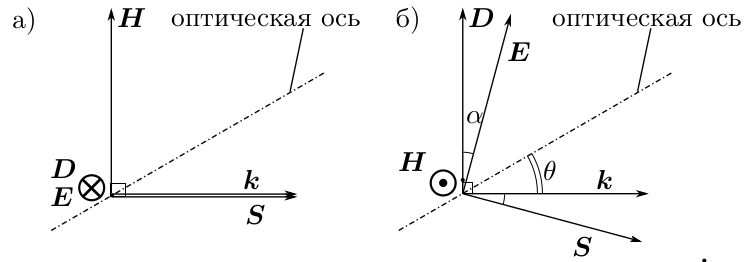
\includegraphics[width = 15cm, height = 5cm]{image1.png}
	\caption{Обыкновенная (а) и необыкновенная (б) волны. Плоскость рисунка --- главное сечение}
\end{figure}
\par
	В первом случае плоская волна называется {\bf обыкновенной}, а во втором --- {\bf необыкновенной} волной. Так как уравнения Максвелла линейны, то в общем случае любое монохроматическое поле в кристалле можно представить в виде суперпозиции обыкновенной и необыкновенной волн.
\par
	Обыкновенная и необыкновенная волны распространяются в кристалле с разной скоростью. Для обыкновенной волны фазовая скорость $v = \omega / k$ не зависит от направления $k$ и равна
\[
	v_o = \frac{c}{\sqrt{\varepsilon_\perp}} = \frac{c}{n_o}.
\]
\par
	У необыкновенной волны векторы индукции и напряжённости электрического поля в общем случае неколлинеарны, а фазовая скорость такой волны зависит от угла $\theta$ между оптической осью и волновым вектором ${\bf k}$
\begin{equation}
	v_e = \frac{c}{\sqrt{\varepsilon}} = \frac{c}{n(\theta)}, \quad \text{где } \varepsilon = \frac{1}{\frac{\sin^2 \theta}{\varepsilon_\parallel} + \frac{\cos^2 \theta}{\varepsilon_\perp}}. \label{extra_v}
\end{equation}
\par
	Таким образом плоская монохроматическая волна, попадающая из изотропной среды в анизотропный одноосный кристалл, распадается в общем случае на две взаимно ортогонально поляризованные плоски волны, распространяющиеся в общем случае в разных направлениях и с разными скоростями.
	
\section*{Теоритическая часть: эффект Поккельса}
\par
	Эффектом Поккельса называется изменение показателя преломления света в кристалле под действием электрического поля, причём это изменение пропорционально напряжённости 
электрического поля. Вследствие эффекта Поккельса в кристалле либо появляется двойное лучепреломление, либо меняется его величина (если кристалл был двулучепреломляющим в отсутствие поля), либо кристалл может стать двуосным.
\par
	Изменение показателя преломления кристаллов под действием внешнего электрического поля происходит за счёт анизотропных свойств кристаллов. Под действием постоянного электрического поля электроны смещаются в сторону того или иного иона, при этом меняется поляризуемость среды и связанный с ней показатель преломления. В первом приближении это изменение линейно относительно внешнего электрического поля. Эффект Поккельса может наблюдаться только в кристаллах, не обладающих центром симметрии.

\section*{Наблюдение интерференционной картины. Экспериментальная установка. Методика измерений.}	
\begin{figure}[h!]
	\centering
	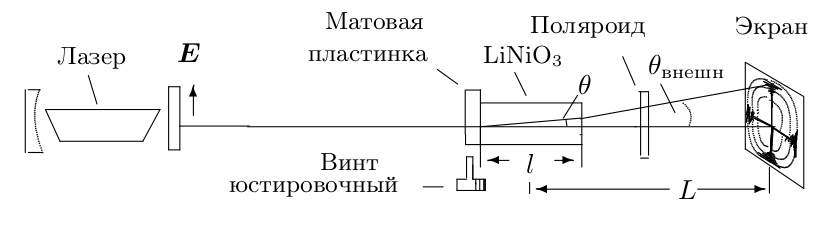
\includegraphics[width = 12cm, height = 5cm]{image2.png}
	\caption{Схема для наблюдения интерференционной картины}
	\label{shm1}	
\end{figure}
\par
	Свет гелий-неонового лазера, поляризованный в вертикальной плоскости, проходя сквозь матовую пластинку, рассевивается и падает на двоякопреломляющий кристалл под различными углами. Кристалл ниобата лития с размерами $3 \times 3 \times 26$ мм вырезан вдоль оптической оси $z$. На экране, расположенном за скрещённом поляроидом, видна интерференционная картина. В нашем эксперименте мы не будем ставить входной поляризатор, так как мы используем лазер, излучение которого поляризовано.
\par
	Благодаря матовой пластинке, после которой лучи рассеиваются под различными углами, на экране, расположенном за поляроидом, мы видим тёмные концетрические окружности --- результат интерференции обыкновенной и необыкновенной волн, или точнее, проекцию их электрических полей на разрешённое направление выходного поляроида.
\par
	Разность фаз между обыкновенной и необыкновенной волнами, приобретаемая при прохожении через кристалл длиной $l$, равна
\[
	\Delta \varphi = \frac{2 \pi}{\lambda} \cdot l \cdot \left( n_o - n(\theta) \right) 
\]
\par
	Если считать, что $n_o$ и $n_e$ отличаются незначительно, для малых углов получим, что
\[
	\Delta \varphi = \frac{2 \pi}{\lambda} l \cdot \left(n_o - n_e \right) \cdot \theta^2.
\]
\par
	Как видим, направлениями постоянной разности фаз служат конусы $\theta = const$, поэтому интерференционная картина представляет собой концентрические окружности. Внутри располагается тёмный крест, который выделяет области, где интерференционная картина отсутствует. В этих направлениях распространяется только одна поляризованная волна (обыкновенная или необыкновенная).
\par
	Для случая, когда разрешённое направление анализатора перпендикулярно поляризации лазерного излучения (скрещённые поляризации), получим выражение для радиуса тёмного кольца с номером $m$:
\begin{equation}
	r_m^2 = \frac{\lambda}{l} \frac{\left(n_o L \right)^2}{\left(n_o - n_e \right)} m, \label{r_main}
\end{equation}
где $L$ --- расстояние от центра кристалла до экрана.
\par
	В данной экспериментальной установке длина волны гелий-неонового лазера $\lambda = 0.63$ мкм, показатель преломления для обыкновенной волны $n_o = 2.29$ считаются известными величинами. Расстояние $L$ было определено с помощью сантиметровой линейки
\[
	L = \left(77.0 \pm 0.5 \right) \, \text{см} \quad \left(\sigma_L = 0.6 \% \right)
\]
\par
	В вертикальной поляризации лазера мы сможем убедиться, если определим разрешённого направление анализатора. Для этого найдём минимум освещенности дневного света, отражённого от поверхности стола. Минимум отражённого света --- вертикальное разрешённое направление поляроида. 
\par
	Соответсвенно, измерив радиусы тёмных колец $r(m)$, мы сможем построить график $r^2 = f(m)$. Определив коэффицент наклона прямой графика $\beta$ с помощью МНК, мы сможем определить двулучепреломление $\left( n_o - n_e \right)$ кристалла ниобата лития c помощью (\ref{r_main}) как
\[
	\left( n_o - n_e \right) = \frac{\lambda}{l} \frac{\left( n_o L \right)^2}{\beta}
\]
\par
	Погрешность $\left( n_o - n_e \right)$ мы сможем найти как
\[
	\Delta_\text{$\left( n_o - n_e \right)$} =  \left( n_o - n_e \right) \cdot \sqrt{( 2\sigma_L)^2 + (\sigma_\beta)^2}
\]
\newpage
\section*{Изучение двойного лучепреломления в электрическом поле. Экспериментальная установка.}
\par
	Если убрать рассеивающую пластинку из установки, схема которой приведена на рис. \ref{shm1} и подать на кристалл постоянное напряжение, то величиной этого напряжения можно будет влиять на поляризацию луча, вышедшего из кристалла. Если заменить экран фотодиодом на той же установке и подать на кристалл переменное напряжение, то можно будет исследовать поляризацию луча с помощью осциллографа. Соотвественная схема экспериментальной установки
\begin{figure}[h!]
	\centering
	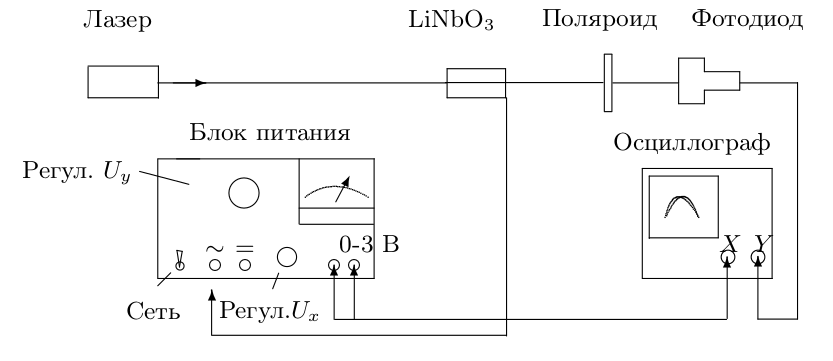
\includegraphics[width = 12cm, height = 5cm]{image3.png}
	\caption{Схема для изучения двойного лучепреломления в электрическом поле}	
\end{figure}
\par
	Рассмотрим случай, когда кристалл помещён в постоянное электрическое поле $E_\text{эл}$, направленное вдоль оси $x$, перпендикулярной оптической оси кристалла $z$. Свойства симметрии кристалла и его электрооптический тензор таковы, что в результате линейного электрооптического эффекта (эффекта Поккельса) в плоскости ($xy$) возникают два главных направления $\xi$ и $\eta$ под углами $45 \degree$ к осям $x$ и $y$ с показателями преломления $(n_o - \Delta n)$ и $(n_o + \Delta n)$, причём $\Delta n = A \cdot E_\text{эл}$, где $A$ --- константа, зависящая только от типа кристалла.
\par
	Возьмём на входе в кристалл вертикально поляризованный свет, а на выходе поставим анализатор, пропускающий горизонтальную поляризацию. Учитывая разложение исходного светового вектора $E = E_0 e^{i(wt-kz)}$ по осям $\xi$ и $\eta$: $E_\xi = E_\eta = E_0 / \sqrt{2}$, запишем разность фаз между векторами $E_\xi$ и $E_\eta$ после прохождения кристалла
\[
	\Delta \varphi = \frac{2 \pi l}{\lambda} 2 \Delta n = \frac{4 \pi l}{\lambda} A E_\text{эл} = \frac{4 \pi}{\lambda} \frac{l}{d} A U,
\]
где $U = E_\text{эл} d$ --- напряжение на кристалле, а $d$ --- размер кристалла в поперечном направлении.
\par
	Результирующее поле анализатора --- сумма проекций $E_\xi$ и $E_\eta$ на направление $x$
\[
	E_\text{вых} = \frac{E_0}{2} e^{i(wt - kl)} \left(e^{i \Delta \varphi / 2} + e^{-i \Delta \varphi / 2} \right) = E_0 e^{i(wt - kl)} \sin\left(\frac{\Delta \varphi}{2} \right)
\]
\newpage
\par
	Отсюда для интенсивности света получим
\begin{equation}
	I_\text{вых} = I_0 \sin^2\left(\frac{\Delta \varphi}{2} \right) = I_0 \sin^2\left(\frac{\pi}{2} \frac{U}{U_\text{$\lambda / 2$}} \right).
\end{equation}
\par
	Здесь введено {\bf полуволновое напряжение}
\begin{equation}
	U_\text{$\lambda / 2$} = \frac{\lambda}{4 A} \frac{d}{l}
\end{equation}
\par
	При $U = U_\text{$\lambda / 2$}$ сдвиг фаз между двумя волнами, соответствующим двум собственным поляризациям, $\Delta \varphi = \pi$, а интенсивность света на выходе анализатора достигает максимума.
\par
	При параллельных поляризациях лазера и анализатора аналогично можно получить, что
\begin{equation}
	I_\text{вых} = I_0 \cos^2\left(\frac{\pi}{2} \frac{U}{U_\text{$\lambda / 2$}} \right).
\end{equation}
\section*{Методика измерений}
\begin{enumerate}
	\item
		Убрав матовую пластинку из установки на рис.2 и подав постоянное напряжение, мы можем проследить как меняется яркость пятна на экране при изменении величины напряжения при скрещенных поляризациях. Исходя из вышеизложенного при $U = U_\text{$\lambda / 2$}$ мы должны наблюдать максимум, а при $U = 2 U_\text{$\lambda / 2$} = U_\text{$\lambda$}$ --- минимум и т.д. При параллельных поляризациях при $U = U_\text{$\lambda / 2$}$ мы должны будем увидеть минимум, а при $U = U_\text{$\lambda$}$ --- максимум. Соответственно, наблюдая за пятном на экране, мы сможем определить полуволновое напряжение ниобата лития по показаниям на блоке питания, где $1.5$ кВ соответствуют $100$ делениям шкалы.
	\item
		Подадим на кристалл напряжение $U = 0.5 U_\text{$\lambda / 2$} = U_\text{$\lambda / 4$}$. Изменим конфигурацию экспериментальной установки: вместо экрана поставим фотодиод и убедимся, что он подключён ко входу $y$ осциллографа, а выход  блока питания подключён к $x$-входу. Таким образом отклонение луча осциллографа по оси $x$ будет пропорционально напряжению $U$ на кристалле, а по оси $y$ --- интенсивности прошедшего через анализатор сигнала  $I_\text{вых}$. Наблюдая на экране фигуры Лиссажу, соответствующие зависимости $I_\text{вых}(U)$ для скрещённых поляризаций лазера и анализатора, определим по фигурам полуволновое напряжение ниобата лития $U = U_\text{$\lambda / 2$}$ как $\Delta U$, соотвествующее переходу от максимума к минимуму сигнала на осциллограмме. При этом будем фиксировать наблюдаемые картины при напряжениях $U_\text{$\lambda / 2$}, U_\text{$\lambda$}$ и $U_\text{$3 \lambda / 2$}$, а также смотреть, как меняются фигуры Лиссажу при переходе к параллельным поляризациям.
\end{enumerate}
\newpage
\section*{Проведённые измерения и полученные результаты}
\subsection*{Наблюдение интерференционной картины. Определение двулучепреломления $(n_o - n_e)$ ниобата лития}
\begin{table}[h!]
	\centering
	\begin{tabular}{|c|c|c|c|}
	\hline
		$r_m$, см & $m$ & ${r_m}^2$, $\text{см}^2$, & $\Delta_\text{${r_m}^2$}$, $\text{см}^2$ \\
	\hline
		2.8 & 1	& 7.84	& 0.28 \\
	\hline
		3.8	& 2	& 14.44	& 0.38 \\
	\hline
		4.7	& 3	& 22.09	& 0.47 \\
	\hline
		5.5	& 4	& 30.25	& 0.55 \\
	\hline
		6.2	& 5	& 38.44	& 0.62 \\
	\hline
		6.8	& 6	& 46.24	& 0.68 \\
	\hline
		7.2	& 7	& 51.84	& 0.72 \\
	\hline
		7.6	& 8	& 57.76	& 0.76 \\
	\hline
		8.1	& 9	& 65.61	& 0.81 \\
	\hline
	\end{tabular}
	\caption{Измерения радиусов тёмных колец $r_m$}
\end{table}
\begin{figure}[h!]
	\centering
	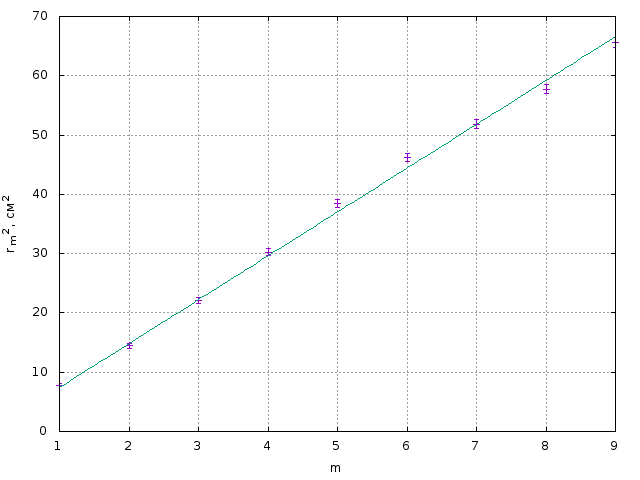
\includegraphics[width = 12cm, height = 7cm]{plot1.png}
	\caption{График зависимости ${r}^2 = f(m)$}	
\end{figure}
\par
	C помощью метода наименьших квадратов найденный коэффициент наклона прямой графика $\beta$:
\[
	\beta = \left(7.40 \pm 0.07 \right) \, \text{см}^2 \quad \left(\sigma_\beta = 1.0 \, \% \right)  
\]
\par
	В результате получим, что двулучепреломление кристалла ниобата лития
\[
	\left(n_o - n_e \right) = \left( 0.1018 \pm 0.0017 \right) \quad \left( \sigma_\text{$\left( n_o - n_e \right)$}  = 1.7 \, \% \right)
\]
\newpage
\par
	Приведём изображения наблюдаемых картин:
\begin{figure}[h!]
	\begin{multicols}{2}
		\hfill
		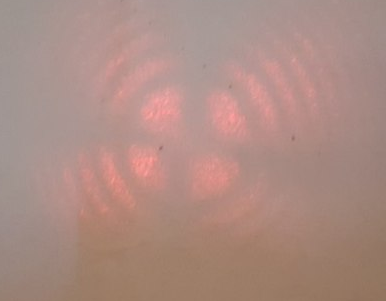
\includegraphics[width = 8cm, height = 5cm]{image5.png}
		\caption{Интерференционная картина при скрещенных поляризациях}
		\hfill
		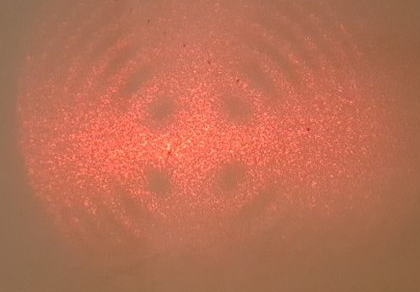
\includegraphics[width = 8cm, height = 5cm]{image6.png}
		\caption{Интерференционная картина при параллельных поляризациях}
		\hfill
	\end{multicols}
\end{figure}

\subsection*{Изучение двойного лучепреломления в электрическом поле. Постоянное напряжение. Определение полуволнового напряжения.}
\par
	Полуволновое напряжение при скрещенных и параллельных поляризациях
\[
	U_\text{$\lambda / 2$} = \left( 450 \pm 8 \right) \, \text{В}
\]
\par
	При скрещенных поляризациях полуволновое напряжение соответствует максимуму яркости наблюдаемого пятна, а при параллельных поляризациях --- минимуму. Обратная ситуация наблюдается при $U = 2 U_\text{$\lambda / 2$}$.

\subsection*{Изучение двойного лучепреломления в электрическом поле. Переменное напряжение. Фигуры Лиссажу.}
\par
	Измерения, проведённые для определения полуволнового напряжения по осциллограмме при скрещенных поляризациях
\begin{table}[h!]
	\centering
	\begin{tabular}{|c|c|c|}
	\hline
		$U_\text{max}$, дел & $U_\text{min}$, дел & $\Delta U$, дел \\
	\hline
		60  & 30 & 30 \\
	\hline
	\end{tabular}
\end{table}
\par
	Полученное полуволновое напряжение
\[
	U_\text{$\lambda / 2$} = \left(450 \pm 11 \right) \, \text{В}
\]
\par
	Отметим, что при переходе к параллельным поляризациям наблюдаемые фигуры Лиссажу инвертируются.
\newpage
\par
	Полученные изображения на экране осциллографа для параллельных поляризаций при напряжениях $U_\text{$\lambda / 2$}, U_\text{$\lambda$}$ и $U_\text{$3 \lambda / 2$}$ соответственно.
\begin{figure}[h!]
	\centering
	\begin{multicols}{3}
		\hfill
		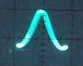
\includegraphics[height = 2.5cm]{image7.png}
		\hfill
		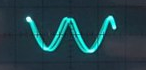
\includegraphics[height = 2.5cm]{image8.png}
		\hfill
		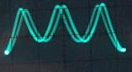
\includegraphics[height = 2.5cm]{image9.png}
		\hfill
	\end{multicols}
\end{figure}

\section*{Выводы}
\par
	Во время работы мы наблюдали на экране интерференционную картину в отсутствие напряжения на кристалле.  Проведя анализ интерференционной картины, мы определили двулучепреломление $n_o - n_e$ ниобата лития
\[
	\left(n_o - n_e \right) = \left( 0.1018 \pm 0.0017 \right) \quad \left( \sigma_\text{$\left( n_o - n_e \right)$}  = 1.7 \, \% \right)
\]	
\par
	Известные табличные значения, соответствующие использованной нами экспериментальной установке: $n_0 = 2.29$, $n_e = 2.20$, и $n_o - n_e = 0.09$.
\par
	Мы также исследовали выходную интенсивность света в зависимости от подаваемого напряжения. В результате мы определили полуволновые напряжения для ниобата лития при скрещенных и параллельных поляризациях, использовав при этом постоянное и переменное напряжения. Важно отметить, что полученные при постоянном и переменном напряжениях значения оказались равными, но были определены с разной точностью.
\par
	Мы также для нескольких характерных напряжений зафиксировали изображения фигур Лиссажу, которые приведены выше.
\end{document}